%%%%%%%%%%%%%%%%%%%%%%%%%%%%%%%%%%%%%%%%%%%%%%%%%%%%%%%
%                   File: OSAmeetings.tex             %
%                  Date: 20 September 2021            %
%                                                     %
%     For preparing LaTeX manuscripts for submission  %
%       submission to Optica meetings and conferences %
%                                                     %
%       (c) 2021 Optica                               %
%%%%%%%%%%%%%%%%%%%%%%%%%%%%%%%%%%%%%%%%%%%%%%%%%%%%%%%

\documentclass[letterpaper,10pt]{article} 
%% if A4 paper needed, change letterpaper to A4

\usepackage{osameet3} %% use version 3 for proper copyright statement

%% standard packages and arguments should be modified as needed
\usepackage{amsmath,amssymb}
\usepackage[colorlinks=true,bookmarks=false,citecolor=blue,urlcolor=blue]{hyperref} %pdflatex
%\usepackage[breaklinks,colorlinks=true,bookmarks=false,citecolor=blue,urlcolor=blue]{hyperref} %latex w/dvipdf
\usepackage[english]{babel}
\newtheorem{theorem}{Theorem}
\newtheorem{corollary}{Corollary}
\newtheorem{lemma}[theorem]{Lemma}
\newtheorem{conjecture}{Conjecture}
\newtheorem{definition}{Definition}
\newtheorem{workdefinition}{Working Definition}
\newtheorem{problem}{Problem}

\usepackage{color}
\newcommand\dashto{\mathrel{
  -\mkern-6mu{\to}\mkern-20mu{\color{white}\bullet}\mkern12mu
}}

\newcommand\indep{\perp \!\!\! \perp}

\usepackage{caption}
\usepackage{subcaption}

\usepackage{tikz} 

%%%%%%%%%%%%%%%%%%%%%%%%%%%%%%%%%%%%%%%%%%%%%%%%%%%%%%%%%%%%%%%%%%%%%%%%%%%%%%%%%%%%%%%

\begin{document}

\title{Inferring Rewards from Discrimination}
% \title{Reward Decomposition of Discrimination}
% \title{Explaining Discrimination by Reward Structure}
% \title{Engineering Fairness through Reward Modification}

\author{Team=\{David Reber\}}
% \address{Columbia University}
% \email{dpr2127@columbia.edu}
%%Uncomment the following line to override copyright year from the default current year.
\copyrightyear{2022}


% \begin{abstract}
% \color{red} TODO: fill in 3 sentence abstract \color{black}
% \end{abstract}

%%%%%%%%%%%%%%%%%%%%%%%%%%%%%%%%%%%%%%%%%%%%%%%%%%%%%%%%%%%%%%%%%%%%%%%%%%%%%%%%%%%%%%%


\section{Personal Background}

\subsection{Relative Academic Strengths}
Relative to the class, I claim a strong and diverse \emph{theoretical} background. Above-average areas, with decreasing \emph{relative} expertise:
\begin{itemize}
  \item \textbf{Mathematical Analysis:} \emph{4 undergraduate courses, 2 graduate courses, master's thesis.} Linear/Nonlinear analysis, metric spaces, complex analysis, spectral theory/calculus, measure theory; manifolds, contraction mappings, Frechet derivative, calculus of variations.
  \item \textbf{Linear Algebra:} \emph{3 undergaduate courses, 1 graduate course, master's thesis}. Linear operators, Banach spaces, all canonical decompositions, pseudospectra/pertubation theory; pseudo-inverses, Perron-Frobenius, iterative methods.
  \item \textbf{Dynamical Systems (discrete):} \emph{1 undergraduate courses, 2 graduate courses, master's thesis.} Linear bounding of nonlinear asymptotics, spectral properties of discrete systems, time-varying systems, time delays; isomorphisms, bifucations, chaos theory.
  \item \textbf{Algorithms:} \emph{3 undergraduate courses, 1 graduate, and I led a competitive coding seminar.} complexity, data structures, theory of computation, recursion, random algorithms.
  \item \textbf{Optimization:} \emph{2 undergraduate courses.} unconstrained, linear, convex, nonlinear constrained, dynamic, combinatorial; KKT, weak/strong duality, Monte Carlo.
  \item \textbf{Machine Learning (theory):} \emph{3 undergraduate courses, 2 graduate courses, 2 years industry.} Kernel-based methods, bayesian methods, stochastic dynamic optimization/reinforcement learning, deep learning, statistical theory (measure theory, Bayesian statistics); value iteration, bandit problems.
\end{itemize}

% Relative to the class average, I claim a strong and diverse \underline{theoretical} background (see Appendix \ref{strengths} for more details): \emph{Mathematical Analysis} (4 undergraduate courses, 2 graduate courses, master's thesis), \emph{Linear Algebra} (3 undergaduate courses, 1 graduate course, master's thesis), \emph{discrete Dynamical Systems} (1 undergraduate courses, 2 graduate courses, master's thesis), \emph{Algorithms} (3 undergraduate courses, 1 graduate, and I led a competitive coding seminar), \emph{Optimization} (2 undergraduate courses), \emph{Machine Learning theory} (3 undergraduate courses, 2 graduate courses, 2 years industry).

\subsection{Non-academic Expertise}
Additionally, I have been interested in anything that can be used to predict agent behavior prior to model training, and causal-based \textbf{agent incentives} seem like a great approach. I've read 3 papers on the topic.

I am well-versed with the latest \textbf{AI safety} research and proposed agendas from academic institutes such as CHAI (Berkeley) and FHI (Oxford), as well as Deepmind, OpenAI, Anthropic, Redwood Research, and MIRI, and I'm becoming increasingly connected with researchers in the field.

I enjoy \textbf{decision theory}; I've read several papers and am well-versed with the variations of Newcomb's paradox and the Prisoner's dillema, L\"{o}b's theorem, and the limitations of CDT and EDT generally. \emph{I would love exploring the cooperative game-theoretic implications of Regret Decision Theory (RDT), theoretically or empirically}.

%%%%%%%%%%%%%%%%%%%%%%%%%%%%%%%%%%%%%%%%%%%%%%%%%%%%%%%%%%%%%%%%%%%%%%%%%%%%%%%%%%%%%%%

\section{Topic and Problem Summary}

This proposal best aligns with the \textbf{Fairness-Discrimination} bucket, and is adjacent to the \textbf{Causal Reinforcement Learning} bucket (see Section \ref{CRL} for discussion).

\subsection{Motivation and Problem Statement}
As algorithms continue to automate systemic decisions (as already attempted with predicted recidivism, loan approval, recruitment/hiring, and academic admissions), there is an increasing need to ensure the fairness of these algorithms. To facilitate better engineering and proactive regulation, we need answers to two questions: 1. What does fairness mean, and 2. How can unfairness be avoided?

R-30 \cite{r30} helps answer the first question, by decomposing the total variation into three distinct measures of counterfactual fairness: $Cft{\text -}DE$, $Cft{\text -}IE$, and $Cft{\text -}SE$. However, these measures are non-identifiable from observational data in many non-markovian settings (i.e. counfounding between a mediator and the decision). Furthermore, while these measures point out where the problem lies with surgical precision, they don't really explain \emph{why} the discrimination occured, and consequently, how to promote future fairness (short of blinding the decision-maker to the sensitive paths, which may not be possible). 

By using response incentives \cite{everitt2021agent, everitt2022understanding} to augment $Cft{\text -}DE$, $Cft{\text -}IE$, and $Cft{\text -}SE$ (here called $Cft$ quantites), this proposal aims to
\begin{itemize}
  \item Identify incentivized $Cft^\uparrow$ quantites from observational distributions, on causal diagrams where (plain) $Cft$ quantites are non-ID. 
  \item Demonstrate that $Cft^\uparrow$ and $Cft^\downarrow$ provide a legitimate decomposition of a $Cft$ measure, so that certain types of reward replacement (e.g. through automation) can be predicted to set $Cft^\downarrow=0$, reducing the overall $Cft$ quantity of interest.
  \item Provide a prodecure for evidencing the reward-dependancies which influenced the decision-maker, to better inform blame attribution and policy adjustment.
\end{itemize}
Note that the final goal is to determine policy and/or reward changes for an agent or institution, based on observed discrimination and causal knowledge (hence the connection to CRL).
Concrete problem statements are included within the research plan of Section \ref{plan}.


%%%%%%%%%%%%%%%%%%%%%%%%%%%%%%%%%%%%%%%%%%%%%%%%%%%%%%%%%%%%%%%%%%%%%%%%%%%%%%%%%%%%%%%

\section{Background: Expressing Reward Incentives in an SCM-framework}

\begin{figure}
\centering
\begin{subfigure}{.5\textwidth}
  \centering
    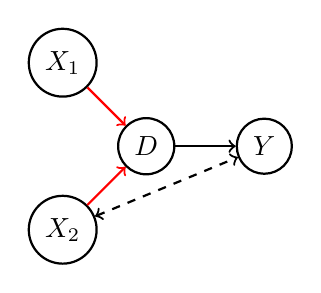
\begin{tikzpicture}[node distance={15mm}, thick, main/.style = {draw, circle}] 
    \node[main] (1) {$X_1$}; 
    \node[main] (2) [below right of=1] {$D$}; 
    \node[main] (3) [below left  of=2] {$X_2$};
    \node[main] (4) [right of=2] {$Y$}; 
    \color{red}\draw[->] (1) -- (2);
    \draw[->] (3) -- (2);
    \color{black}\draw[->] (2) -- (4);
    \draw[dashed,<->] (3) -- (4);
    \end{tikzpicture}
  \caption{Direct effect of $\mathbf{X}=\{X_1,X_2\}$ on $D$}
  \label{fig:direct}
\end{subfigure}%
\begin{subfigure}{.5\textwidth}
  \centering
    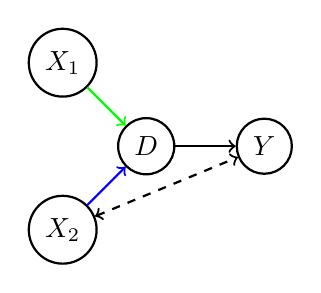
\begin{tikzpicture}[node distance={15mm}, thick, main/.style = {draw, circle}] 
    \node[main] (1) {$X_1$}; 
    \node[main] (2) [below right of=1] {$D$}; 
    \node[main] (3) [below left  of=2] {$X_2$};
    \node[main] (4) [right of=2] {$Y$}; 
    \color{green}\draw[->] (1) -- (2);
    \color{blue}\draw[->] (3) -- (2);
    \color{black}\draw[->] (2) -- (4);
    \draw[dashed,<->] (3) -- (4);
    \end{tikzpicture}
  \caption{Decomposition of the direct effect of $\mathbf{X}$ on $D$}
  \label{fig:decomp}
\end{subfigure}
\caption{A simple example of an incentives decomposition of the direct effect of $\mathbf{X}$ on $D$, as rewarded by $Y$.}
\label{fig:simple}
\end{figure}

The following notation and definitions help keep consistency with the lab's existing work on both fairness\cite{r30} and CRL \cite{r57} (see Figure \ref{fig:direct} for a visual aid). In addition to the usual SCM $M=(V,U,F,P(U))$, we use $Y$ as the reward variable(s), $D\in An(Y)$ as the decision node, and $X\in An(D)$ as the sensitive attribute(s) which the decision may be unfair towards. $\mathbf{C}\subset V$ are the covariates which $D$ is allowed to observe; that is, $Pa(D)\subset \mathbf{C}$. A policy $\pi$ is a soft intervention on $D$ which respects $domain(\pi)\subset \mathbf{C}\cup \{U_D\}$, and an \emph{optimal policy} is defined as a policy $\pi$ that maximizes the sum of the expected rewards: $\mathbb{E}_\pi [\sum_{Y\in\mathbf{Y}}Y]$.
Lastly, a `fairness effect $E$' is just some element $E\in\{Cft{\text -}DE,\hspace{2mm} Cft{\text -}IE,\hspace{2mm} Cft{\text -}SE\}$.

\begin{definition}[Response Incentive]
Let $M=(V,U,F,P(U))$ be an SCM. A policy $\pi$ responds to a variable $X\in V$ if there exists some intervention $do(X=x)$ and some exogenous unit $U=u$, such that $D_x(u) \neq D(u)$. The variable $X$ has an \emph{response incentive} if all optimal policies respond to $X$.
We say a causal diagram $G$ \emph{admits} an response incentive on $X$ if it is compatible with an SCM that has an response incentive on $X$.
\end{definition}

Note that \emph{response incentive} is a binary classification of the ancestors of $D$: either a node has an response incentive, or it doesn't.
Next, the \emph{minimal reduction} of a causal graph $G$ eliminates all edges from parents of $D$ which do not have their own d-connection to $Y$.

\begin{definition}[Minimal Reduction]
The \emph{minimal reduction} $G^{min}$ of a causal diagram $G$ is the result of removing from $G$ all edges $X\rightarrow D$ satisfying $(X\indep Y | D \cup Pa(D) \setminus X)$.
\end{definition}

Intuitively, the minimal reduction breaks all non-informative links to the decision node.
The main result from \cite{everitt2021agent} we build on is a graphical criterion for classifying a node $X$ as having an response incentive.


\begin{theorem}[Markovian Case: Response Incentive Criterion \cite{everitt2021agent}]\label{markov}
Let $G$ be a Markovian causal diagram. Then $G$ admits a response incentive on $X\in V$ if and only if the minimal reduction $G^{min}$ has a directed path $X\dashto D$.
\end{theorem}

\begin{definition}[Incentivized Discrimination]
Let $G$ be a causal diagram, with $X$, $D$, and $Y$ as previously defined. Let $E$ be some measure of a discriminatory effect $X$ on $D$. The \emph{incentivized effect} $E^\uparrow$, of $X$ on $D$ with respect to $Y$, is defined as the value of $E$ on $G^{min}$. 
\end{definition}

For example, consider the counterfactual direct effect $Cft{\text -}DE(X,D)$  of $X$ on $D$. Then $Cft{\text -}DE^\uparrow(X,D,Y)$ is obtained by first finding $G^{min}$ (which is defined only relative to $Y$), then computing the $Cft{\text -}DE$ effect in this reduced graph (see Figure \ref{grades}).

\begin{figure}[htbp]
\centerline{\includegraphics[width=0.5\textwidth]{pics/grade_prediction.png}}
\caption{Source: \cite{everitt2021agent}. Here, discrimination is incentivized with respect to Race, but not incentivized with respect to Gender, because the edge from Gender is eliminated in $G^{min}$.}
\label{grades}
\end{figure}

%%%%%%%%%%%%%%%%%%%%%%%%%%%%%%%%%%%%%%%%%%%%%%%%%%%%%%%%%%%%%%%%%%%%%%%%%%%%%%%%%%%%%%%

\section{Research Plan and Preliminary Work}\label{plan}
The first step will be to extend Theorem \ref{markov} to the Non-Markovian case: this is foundational for the following directions. (It seems trivial if confounding is not allowed on $D$, but then we wouldn't be able to say anything about the Berkeley admissions case).

\subsection{Identifying Incentivized Discrimination}
The identification problem of the $Cft$ quantities is strictly easier when incentives are taken into account, since the reduced graph $G^{min}$ is obtained by removing edges from $G$. I conjecture there will be nontrivial families of graphs for which $Cft{\text -}DE$, $Cft{\text -}IE$, and $Cft{\text -}SE$ are not identifiable from observational distributions, but for which $Cft{\text -}DE^\uparrow$, $Cft{\text -}IE^\uparrow$, and/or $Cft{\text -}SE^\uparrow$ are always identifiable. 

\begin{problem}{Identification of Incentifized Cft quantities}\label{cft-id}

\textbf{Inputs:} $G$, $P(V)$, and an incentivised effect $E^\uparrow\in\{Cft{\text -}DE^\uparrow,\hspace{2mm} Cft{\text -}IE^\uparrow,\hspace{2mm} Cft{\text -}SE^\uparrow\}$

\textbf{Outputs:} Yes/No (Is $E^\uparrow$ ID from $G$ and $P(V)$)
\end{problem}




\subsection{Incentives-based Decomposition of Discrimatory Effects}
\begin{conjecture}[Unincentivized Null]\label{null-conj}
Let $G$ be a causal diagram, with $X$, $D$, and $Y$ as previously defined. Suppose $(X\indep Y | D \cup Pa(D) \setminus X)$.

Then $Cft{\text -}DE^\uparrow (X,D) = 0$.

(Epistemic status: Almost certain. I speculate that there may be similar results about $Cft{\text -}IE^\uparrow (X,D)$ and $Cft{\text -}SE^\uparrow (X,D)$, but I'm less confident about those.)
\end{conjecture}

If our models and data were perfect, and our policies optimal in maximizing rewards, then (assuming Conjecture \ref{null-conj} holds) we will observe that $Cft{\text -}DE^\uparrow (X,D) = 0$. But what if our model is mispecified, our data is noisy, or our policies are sub-optimal for maximizing our reward $Y$? Then our null result won't be exactly zero; perhaps only close to zero.

How might we measure the magnitude of this `unincentivized' effect from data, when theoretically it should be zero? Here's a possible working definition:

\begin{workdefinition}[Unincentivized Discrimination]
Let $G$ be a causal diagram, with $\mathbf{X}$ containing multiple sensitive attributes. Partition $\mathbf{X}=\mathbf{X}^\uparrow\cup \mathbf{X}^\downarrow$, where $\mathbf{X}^\downarrow:=\{X\in An(D)| (X\indep Y | D \cup Pa(D) \setminus X)\}$ and $\mathbf{X}^\uparrow:=\mathbf{X}\setminus\mathbf{X}^\downarrow$. 

Let $E(X,D)$ be some fairness measure of a discriminatory effect $X$ on $D$. The \emph{unincentivized effect} $E^\downarrow(\mathbf{X},D,Y)$, of $X$ on $D$ with respect to $Y$, is defined as
\[
E^\downarrow(\mathbf{X},D,Y) := E(\mathbf{X}^\downarrow,D)
\] 
\end{workdefinition}

Note that Conjecture \ref{null-conj} could now be expressed as saying that $Cft{\text -}DE^\downarrow(\mathbf{X},D,Y)=0$ (if our models and data are perfect and our policies are optimal in maximizing rewards).


No matter what definition of `Unincentived Discrimination' we use, we want to ensure that it's physically (and intuitively) meaningful; that is, the `incentivized' and `unincentivized' portions of the $Cft{\text -}DE$ effect should form a \textbf{decomposition} of the total value of the $Cft{\text -}DE$ effect.

\begin{problem}{Incentivized Decomposition of Discrimination}

\textbf{Inputs:} An incentivised effect $E\in\{Cft{\text -}DE,\hspace{2mm} Cft{\text -}IE,\hspace{2mm} Cft{\text -}SE\}$

\textbf{Outputs:} A function $g$ satisfying $E(\mathbf{X},D,Y)=g(E^\uparrow(\mathbf{X},D,Y),E^\downarrow(\mathbf{X},D,Y))$ (which holds across all $G$ and $P(V)$)
\end{problem}

\begin{conjecture}[Decomposition of Discrimantory Effect]\label{decomp-conj}
$E(\mathbf{X},D,Y) = E^\uparrow(\mathbf{X},D,Y) + E^\downarrow(\mathbf{X},D,Y)$.

(Epistemic status: Somewhat confident. I think it's more likely to hold in the linear case, at any rate).
\end{conjecture}




\subsection{Explaining Discrimination via Rewards}
If we have discriminatory data and a causal diagram, we would like to be able to assign likelihoods to the various reward structures which could explain the discrimination.


\begin{problem}{Evidence of Reward}\label{reward-id}

\textbf{Inputs:} $G_Y$ ($G$ with node $Y$ removed), $P(V)$, $Pa(\hat{Y})$ (a candidate set of $Y$'s parents), and a value for $E(X,D)$ (where $E\in\{Cft{\text -}DE,\hspace{2mm} Cft{\text -}IE,\hspace{2mm} Cft{\text -}SE\}$)

\textbf{Outputs:} Fraction of $E(X,D)$ explainable by $Pa(\hat{Y})$
\end{problem}

Note that for a given dataset and casual diagram $G$, the value of $Cft{\text -}DE^\downarrow(\mathbf{X},D,Y)$ is dependent on the structural assumptions of $Y$: in particular, on the dependencies that $Y$ has. 

Suppose that, for proprietary or historical reasons, we do not know $Y$'s dependancies (as in Figure \ref{fig:berkeley}). In this case, perhaps we can use $Cft{\text -}DE^\downarrow(\mathbf{X},D,Y)$ as evidence for whether our modeling choice of $Y$ is valid, since if $Cft{\text -}DE^\downarrow(\mathbf{X},D,Y)<Cft{\text -}DE^\downarrow(\mathbf{X},D,Y^\prime)$, then presumably the reward $Y$ is explaining more of the discrimination than $Y^\prime$ is. Formally:

\begin{conjecture}[Reward Identification]\label{decomp-conj}
Let $G$, $P(V)$ be given, with $\mathbf{X}$ and $D$ specified. Assume $P(V)$ was generated by an optimal policy $\pi^*$ w.rt. the true, unknown reward function $f_{Y^*}$. Then $Pa(\hat{Y})\subset Pa(Y^*)$, where $\hat{Y}$ satisfies
\[
\hat{Y} = \arg \min_Y \quad Cft{\text -}DE^\downarrow(\mathbf{X},D,Y)
\]
If $f_{Y^*}$ has no trivial dependancies, then $Pa(Y^*)=Pa(\hat{Y})$

(Epistemic status: Likely.
I suspect `trivial dependencies' are important to consider, but I recognize that's a hand-wavy term. I'm trying to convey that $Y^*$ and $\hat{Y}$ share the same dependencies, and there may be ways to express that other than $Pa(\hat{Y})=Pa(Y^*)$).
\end{conjecture}

I would like to test Conjecture \ref{decomp-conj} numerically using synthetic datasets first, to first get a sense for its usefulness (since it seems likely that noisy data, or a suboptimal policy, might render such a conjecture useless in a practical sense).

% Furthermore, if $Cft{\text -}IE^\downarrow$ and $Cft{\text -}SE^\downarrow$ are also well-defined, then perhaps there's tradeoffs to minimizing these three measures simultaneously. Perhaps we try to minimize all together. I think a weighted cost function would have a meaningful value (like, penalizing $Cft{\text -}IE^\downarrow$ half as much as either $Cft{\text -}SE^\downarrow$ or $Cft{\text -}DE^\downarrow$ for situations where indirect variation is acceptable but still somewhat undesirable by societal norms).

% Lastly, I suspect that 

% \begin{conjecture}[Reward Decomposition]\label{reward-decom}
% Let $G$, $P(V)$ be given, with $\mathbf{X}$ and $D$ specified. Assume $P(V)$ was generated by an optimal policy $\pi^*$ w.rt. the true, unknown reward function $f_{Y^*}$. Then $Pa(\hat{Y})\subset Pa(Y^*)$, where $\hat{Y}$ satisfies
% \[
% \hat{Y} = \arg \min_Y \quad Cft{\text -}DE^\downarrow(\mathbf{X},D,Y)
% \]
% If $f_{Y^*}$ has no trivial dependancies, then $Pa(Y^*)=Pa(\hat{Y})$

% (Epistemic status: Plausible, but speculative.
% I suspect `trivial dependencies' are important to consider, but I recognize that's a hand-wavy term. I'm trying to convey that $Y^*$ and $\hat{Y}$ share the same dependencies, and there may be ways to express that other than $Pa(\hat{Y})=Pa(Y^*)$).
% \end{conjecture}

\begin{figure}
\centering
\begin{subfigure}{.5\textwidth}
  \centering
  \includegraphics[width=.8\linewidth]{pics/berkeley_A.png}
  \caption{Reward $Y_2$ which does not incentivize bias}
  \label{fig:berkeley_fair}
\end{subfigure}%
\begin{subfigure}{.5\textwidth}
  \centering
  \includegraphics[width=.8\linewidth]{pics/berkeley_B.png}
  \caption{Reward $Y_2$ which does incentivize gender bias}
  \label{fig:berkeley_unfair}
\end{subfigure}
\caption{Source: \cite{everitt2022understanding}. Using our notation, $X=$`Gender', $D=$`Admit', $Y_1=$`Student performance', and either $Y_2=$`Right number of students' or $Y_2=$`percent men'. Although the reward is not known to us, we can infer its structure based on how well it matches the discrimination.}
\label{fig:berkeley}
\end{figure}


\section{Relation to CRL}\label{CRL}
Ultimately, the goal of this research direction is to predict fairness attributes of an ML architecture prior to training, to make `being fair' easier to engineer, and easier to regulate. But, this is only possible given some degree of causal knowledge about the feature space (and the reward function, but that's engineered).

I expect these results to evidence that CRL is inherently easier to align with what we want (such as `fairness') than non-causal RL. However, it is not immediately clear to me how addressing any of these problems can improve performance/training, unfortunately. 

I was surprised to realize that Problem \ref{reward-id} is very similar to causal imitation learning: the difference is that instead of trying to learn an agent's policy, we are trying to infer some information about about agent's reward structure. 

Meanwhile, addressing Problem \ref{cft-id} \emph{may} enable $Cft{\text -}DE$,\hspace{1pt} $Cft{\text -}IE$ and $Cft{\text -}SE$ to be used more readily as regularization functions.


%%%%%%%%%%%%%%%%%%%%%%%%%%%%%%%%%%%%%%%%%%%%%%%%%%%%%%%%%%%%%%%%%%%%%%%%%%%%%%%%%%%%%%%

\newpage
% \bibliography{dressing_room} 
\begin{thebibliography}{99} %% use BibTeX or add references manually

\bibitem{r30}
J. Zhang, E. Bareinboim,
``Fairness in Decision-Making – The Causal Explanation Formula'',
AAAI-18. In Proceedings of the 32nd AAAI Conference on Artificial Intelligence, 2018.
Columbia CausalAI Laboratory, Technical Report (R-30), Nov, 2017.
\url{https://causalai.net/r30.pdf}

\bibitem{r57}
J. Zhang, E. Bareinboim,
``Designing Optimal Dynamic Treatment Regimes: A Causal Reinforcement Learning Approach'', ICML-20. In Proceedings of the 37th International Conference on Machine Learning, 2020.
Columbia CausalAI Laboratory, Technical Report (R-57), Jun, 2020. 
\url{https://causalai.net/r57.pdf}

\bibitem{everitt2021agent}
T. Everitt, R. Carey, E. D. Langlois, P. A. Ortega, S. Legg,
``Agent Incentives: A Causal Perspective,''
in \emph{Proceedings of the AAAI 2021 Conference}, 
arXiv:2102.01685v2 [cs.AI], 2021.
\url{https://arxiv.org/abs/2102.01685v2}

\bibitem{everitt2022understanding}
T. Everitt, P. A. Ortega, E. Barnes, S. Legg,
``Understanding Agent Incentives using Causal Influence Diagrams. Part I: Single Action Settings,'' arXiv:1902.09980v7 [cs.AI], 2022.
\url{https://arxiv.org/abs/1902.09980v7}


% \bibitem{b6} Y. Yorozu, M. Hirano, K. Oka, and Y. Tagawa, ``Electron spectroscopy studies on magneto-optical media and plastic substrate interface,'' IEEE Transl. J. Magn. Japan, vol. 2, pp. 740--741, August 1987 [Digests 9th Annual Conf. Magnetics Japan, p. 301, 1982].

% \bibitem{craig96} R. Craig and B. Gignac, ``High-power 980-nm pump lasers,''
% in \emph{Optical Fiber Communication Conference}, Vol. 2 of 1996 OSA Technical Digest Series (Optical Society of America, 1996), paper ThG1.



% %%%%%%%%%%%%%% DEMO REERENCES %%%%%%%%%%%%%%%%%%%%%

% \bibitem{b1} G. Eason, B. Noble, and I. N. Sneddon, ``On certain integrals of Lipschitz-Hankel type involving products of Bessel functions,'' Phil. Trans. Roy. Soc. London, vol. A247, pp. 529--551, April 1955.
% \bibitem{b2} J. Clerk Maxwell, A Treatise on Electricity and Magnetism, 3rd ed., vol. 2. Oxford: Clarendon, 1892, pp.68--73.
% \bibitem{b3} I. S. Jacobs and C. P. Bean, ``Fine particles, thin films and exchange anisotropy,'' in Magnetism, vol. III, G. T. Rado and H. Suhl, Eds. New York: Academic, 1963, pp. 271--350.
% \bibitem{b4} K. Elissa, ``Title of paper if known,'' unpublished.
% \bibitem{b5} R. Nicole, ``Title of paper with only first word capitalized,'' J. Name Stand. Abbrev., in press.
% \bibitem{b6} Y. Yorozu, M. Hirano, K. Oka, and Y. Tagawa, ``Electron spectroscopy studies on magneto-optical media and plastic substrate interface,'' IEEE Transl. J. Magn. Japan, vol. 2, pp. 740--741, August 1987 [Digests 9th Annual Conf. Magnetics Japan, p. 301, 1982].
% \bibitem{b7} M. Young, The Technical Writer's Handbook. Mill Valley, CA: University Science, 1989.

% %%%%%%%%%%%%%% DEMO REERENCES %%%%%%%%%%%%%%%%%%%%%%

% \bibitem{krishnan00} E. Krishnan, A. M. Shan, T. Rishi, L. A. Ajith, C. V.
% Radhakrishnan, \textit{On-line Tutorial on \LaTeX{}},
% ``Mathematics'' (Indian \TeX{} Users Group, 2000), \\
% \url{http://www.tug.org/tutorials/tugindia/chap11-scr.pdf}.

% \bibitem{vantrigt97} C. van Trigt, ``Visual system-response functions and estimating reflectance,''
% J. Opt. Soc. Am. A \textbf{14}, 741--755 (1997).

% \bibitem{masters93} T. masters, \emph{Practical Neural Network Recipes in C++} (Academic, 1993).

% \bibitem{shoop97} B. L. Shoop, A. H. Sayles, and D. M. Litynski, ``New devices for optoelectronics: smart pixels,''
% in \emph{Handbook of Fiber Optic Data Communications},
% C. DeCusatis, D. Clement, E. Maass, and R. Lasky, eds. (Academic, 1997), pp. 705--758.

% \bibitem{kalman76} R. E. Kalman,``Algebraic aspects of the generalized inverse of a rectangular matrix,'' in
% \emph{Proceedings of Advanced Seminar on Generalized Inverse and Applications}, M. Z. Nashed, ed. (Academic, 1976), pp. 111--124.

% \bibitem{craig96} R. Craig and B. Gignac, ``High-power 980-nm pump lasers,''
% in \emph{Optical Fiber Communication Conference}, Vol. 2 of 1996 OSA Technical Digest Series (Optical Society of America, 1996), paper ThG1.

% \bibitem{steup96} D. Steup and J. Weinzierl, ``Resonant THz-meshes,''
% presented at the Fourth International Workshop on THz Electronics, Erlangen-Tennenlohe, Germany, 5--6 Sept. 1996.

\end{thebibliography}

%%%%%%%%%%%%%%%%%%%%%%%%%%%%%%%%%%%%%%%%%%%%%%%%%%%%%%%%%%%%%%%%%%%%%%%%%%%%%%%%%%%%%%%

% \section{Appendix}

% % \color{red}
% % your project proposal should have 1-2 pages listing the chosen topic (possibly among the buckets in the course's webpage), a title, a clear problem statement (input-output), possibly some evidence of preliminary work (e.g., educated conjectures), and relevant references. 
% %  \color{black}

% \subsection{Elaboration on Strengths}\label{strengths}
% More detail about my strengths, to avoid confusion:
% % \begin{itemize}
% %   \item \textbf{Mathematical Analysis:} Linear/Nonlinear analysis, metric spaces, complex analysis, spectral theory/calculus, measure theory; manifolds, contraction mappings, Frechet derivative, calculus of variations.
% %   \item \textbf{Linear Algebra:} Linear operators, Banach spaces, all canonical decompositions, pseudospectra/pertubation theory; pseudo-inverses, Perron-Frobenius, iterative methods.
% %   \item \textbf{Dynamical Systems (discrete):} Linear bounding of nonlinear asymptotics, spectral properties of discrete systems, time-varying systems, time delays; isomorphisms, bifucations, chaos theory.
% %   \item \textbf{Algorithms:} complexity, data structures, theory of computation, recursion, random algorithms.
% %   \item \textbf{Optimization:} unconstrained, linear, convex, nonlinear constrained, dynamic, combinatorial; KKT, weak/strong duality, Monte Carlo.
% %   \item \textbf{Machine Learning (theory):} Kernel-based methods, bayesian methods, stochastic dynamic optimization/reinforcement learning, deep learning, statistical theory (measure theory, Bayesian statistics); value iteration, bandit problems.
% % \end{itemize}


% \begin{itemize}
%   \item \textbf{Mathematical Analysis:} \emph{4 undergraduate courses, 2 graduate courses, master's thesis.} Linear/Nonlinear analysis, metric spaces, complex analysis, spectral theory/calculus, measure theory; manifolds, contraction mappings, Frechet derivative, calculus of variations.
%   \item \textbf{Linear Algebra:} \emph{3 undergaduate courses, 1 graduate course, master's thesis}. Linear operators, Banach spaces, all canonical decompositions, pseudospectra/pertubation theory; pseudo-inverses, Perron-Frobenius, iterative methods.
%   \item \textbf{Dynamical Systems (discrete):} \emph{1 undergraduate courses, 2 graduate courses, master's thesis.} Linear bounding of nonlinear asymptotics, spectral properties of discrete systems, time-varying systems, time delays; isomorphisms, bifucations, chaos theory.
%   \item \textbf{Algorithms:} \emph{3 undergraduate courses, 1 graduate, and I led a competitive coding seminar.} complexity, data structures, theory of computation, recursion, random algorithms.
%   \item \textbf{Optimization:} \emph{2 undergraduate courses.} unconstrained, linear, convex, nonlinear constrained, dynamic, combinatorial; KKT, weak/strong duality, Monte Carlo.
%   \item \textbf{Machine Learning (theory):} \emph{3 undergraduate courses, 2 graduate courses, 2 years industry.} Kernel-based methods, bayesian methods, stochastic dynamic optimization/reinforcement learning, deep learning, statistical theory (measure theory, Bayesian statistics); value iteration, bandit problems.
% \end{itemize}

\end{document}
